\documentclass[12pt]{article}
\usepackage[utf8]{inputenc}
\usepackage{graphicx}
\usepackage{geometry}
\geometry{a4paper, margin=0.8in}

\title{Hospital Management System: Final Stage }
\author{Muhammad Rehan \\ 22P-9106}
\date{Assignment 04}

\begin{document}
\maketitle

\begin{abstract}
This assignment has enhancements made to the Hospital Management System (HMS) in Stage 4, focusing on the implementation of SOLID design principles to improve the system’s design and architecture. This assignment addresses improvements in modularity, maintainability, and scalability by refining class structures and interactions within the system. Detailed explanations of the adjustments in class diagrams and sequence diagrams illustrate the practical application of these principles.
\end{abstract}

\section*{Introduction}
In the previous assignment of HMS, the initial design and sequence diagrams were developed, capturing basic functionalities and interactions. Assignment 4 advances this design by applying SOLID principles, which are fundamental to creating a more robust, maintainable, and flexible object-oriented system. These principles guide the restructuring and enhancement of the system architecture.

\section*{Application of SOLID Principles}
\subsection*{Overview of SOLID Principles}
SOLID principles, which I've used in this assignment, consist of five design principles intended to make software designs more understandable, flexible, and maintainable:
\begin{itemize}
    \item \textbf{Single Responsibility Principle (SRP)}: A class should have only one reason to change.
    \item \textbf{Open/Closed Principle (OCP)}: Objects or entities should be open for extension but closed for modification.
    \item \textbf{Liskov Substitution Principle (LSP)}: Objects of a superclass shall be replaceable with objects of its subclasses without affecting the application.
    \item \textbf{Interface Segregation Principle (ISP)}: Many client-specific interfaces are better than one general-purpose interface.
    \item \textbf{Dependency Inversion Principle (DIP)}: High-level modules should not depend on low-level modules. Both should depend on abstractions.
\end{itemize}

\section*{Enhanced Class Diagram}
The enhanced class diagram, shown below, illustrates the refined structure and relationships, emphasizing adherence to SOLID principles.

\begin{figure}[h!]
\centering
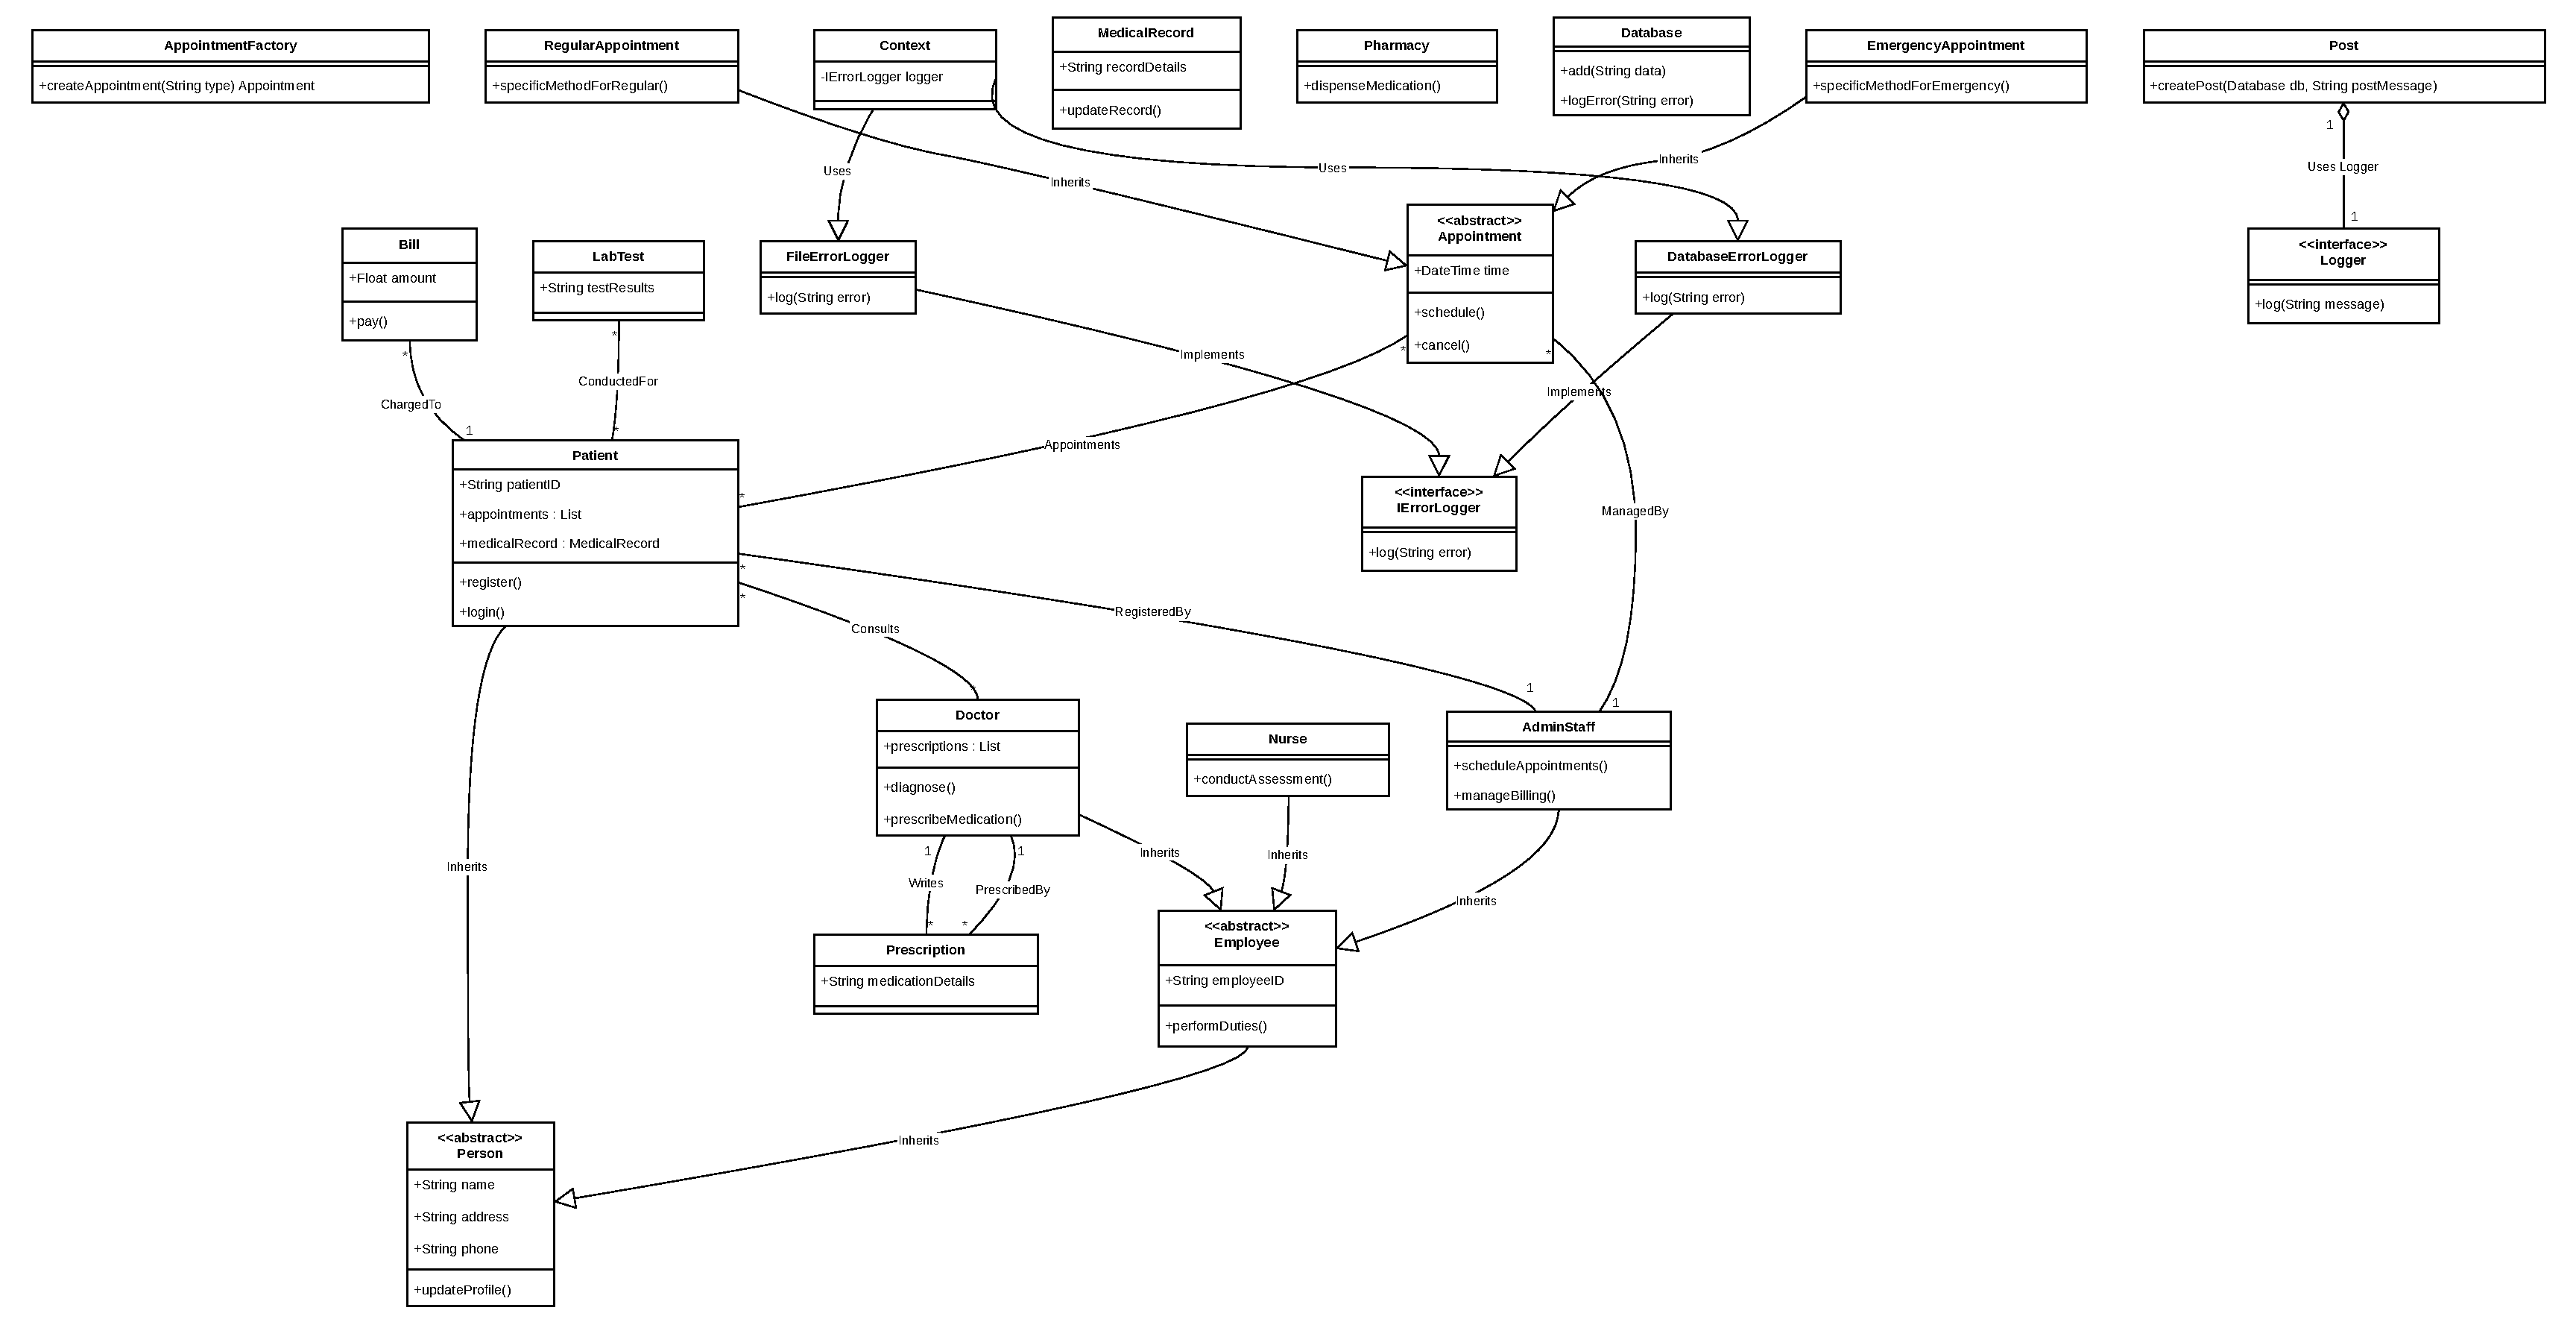
\includegraphics[width=1\textwidth]{new_class.pdf} % Updated file name after conversion
\caption{Enhanced Class Diagram incorporating SOLID principles}
\end{figure}

\section*{Updated Sequence Diagrams}
Following are the revised sequence diagrams, showcasing the application of SOLID principles in system interactions.

\subsection*{Booking an Appointment}
\begin{figure}[h!]
\centering
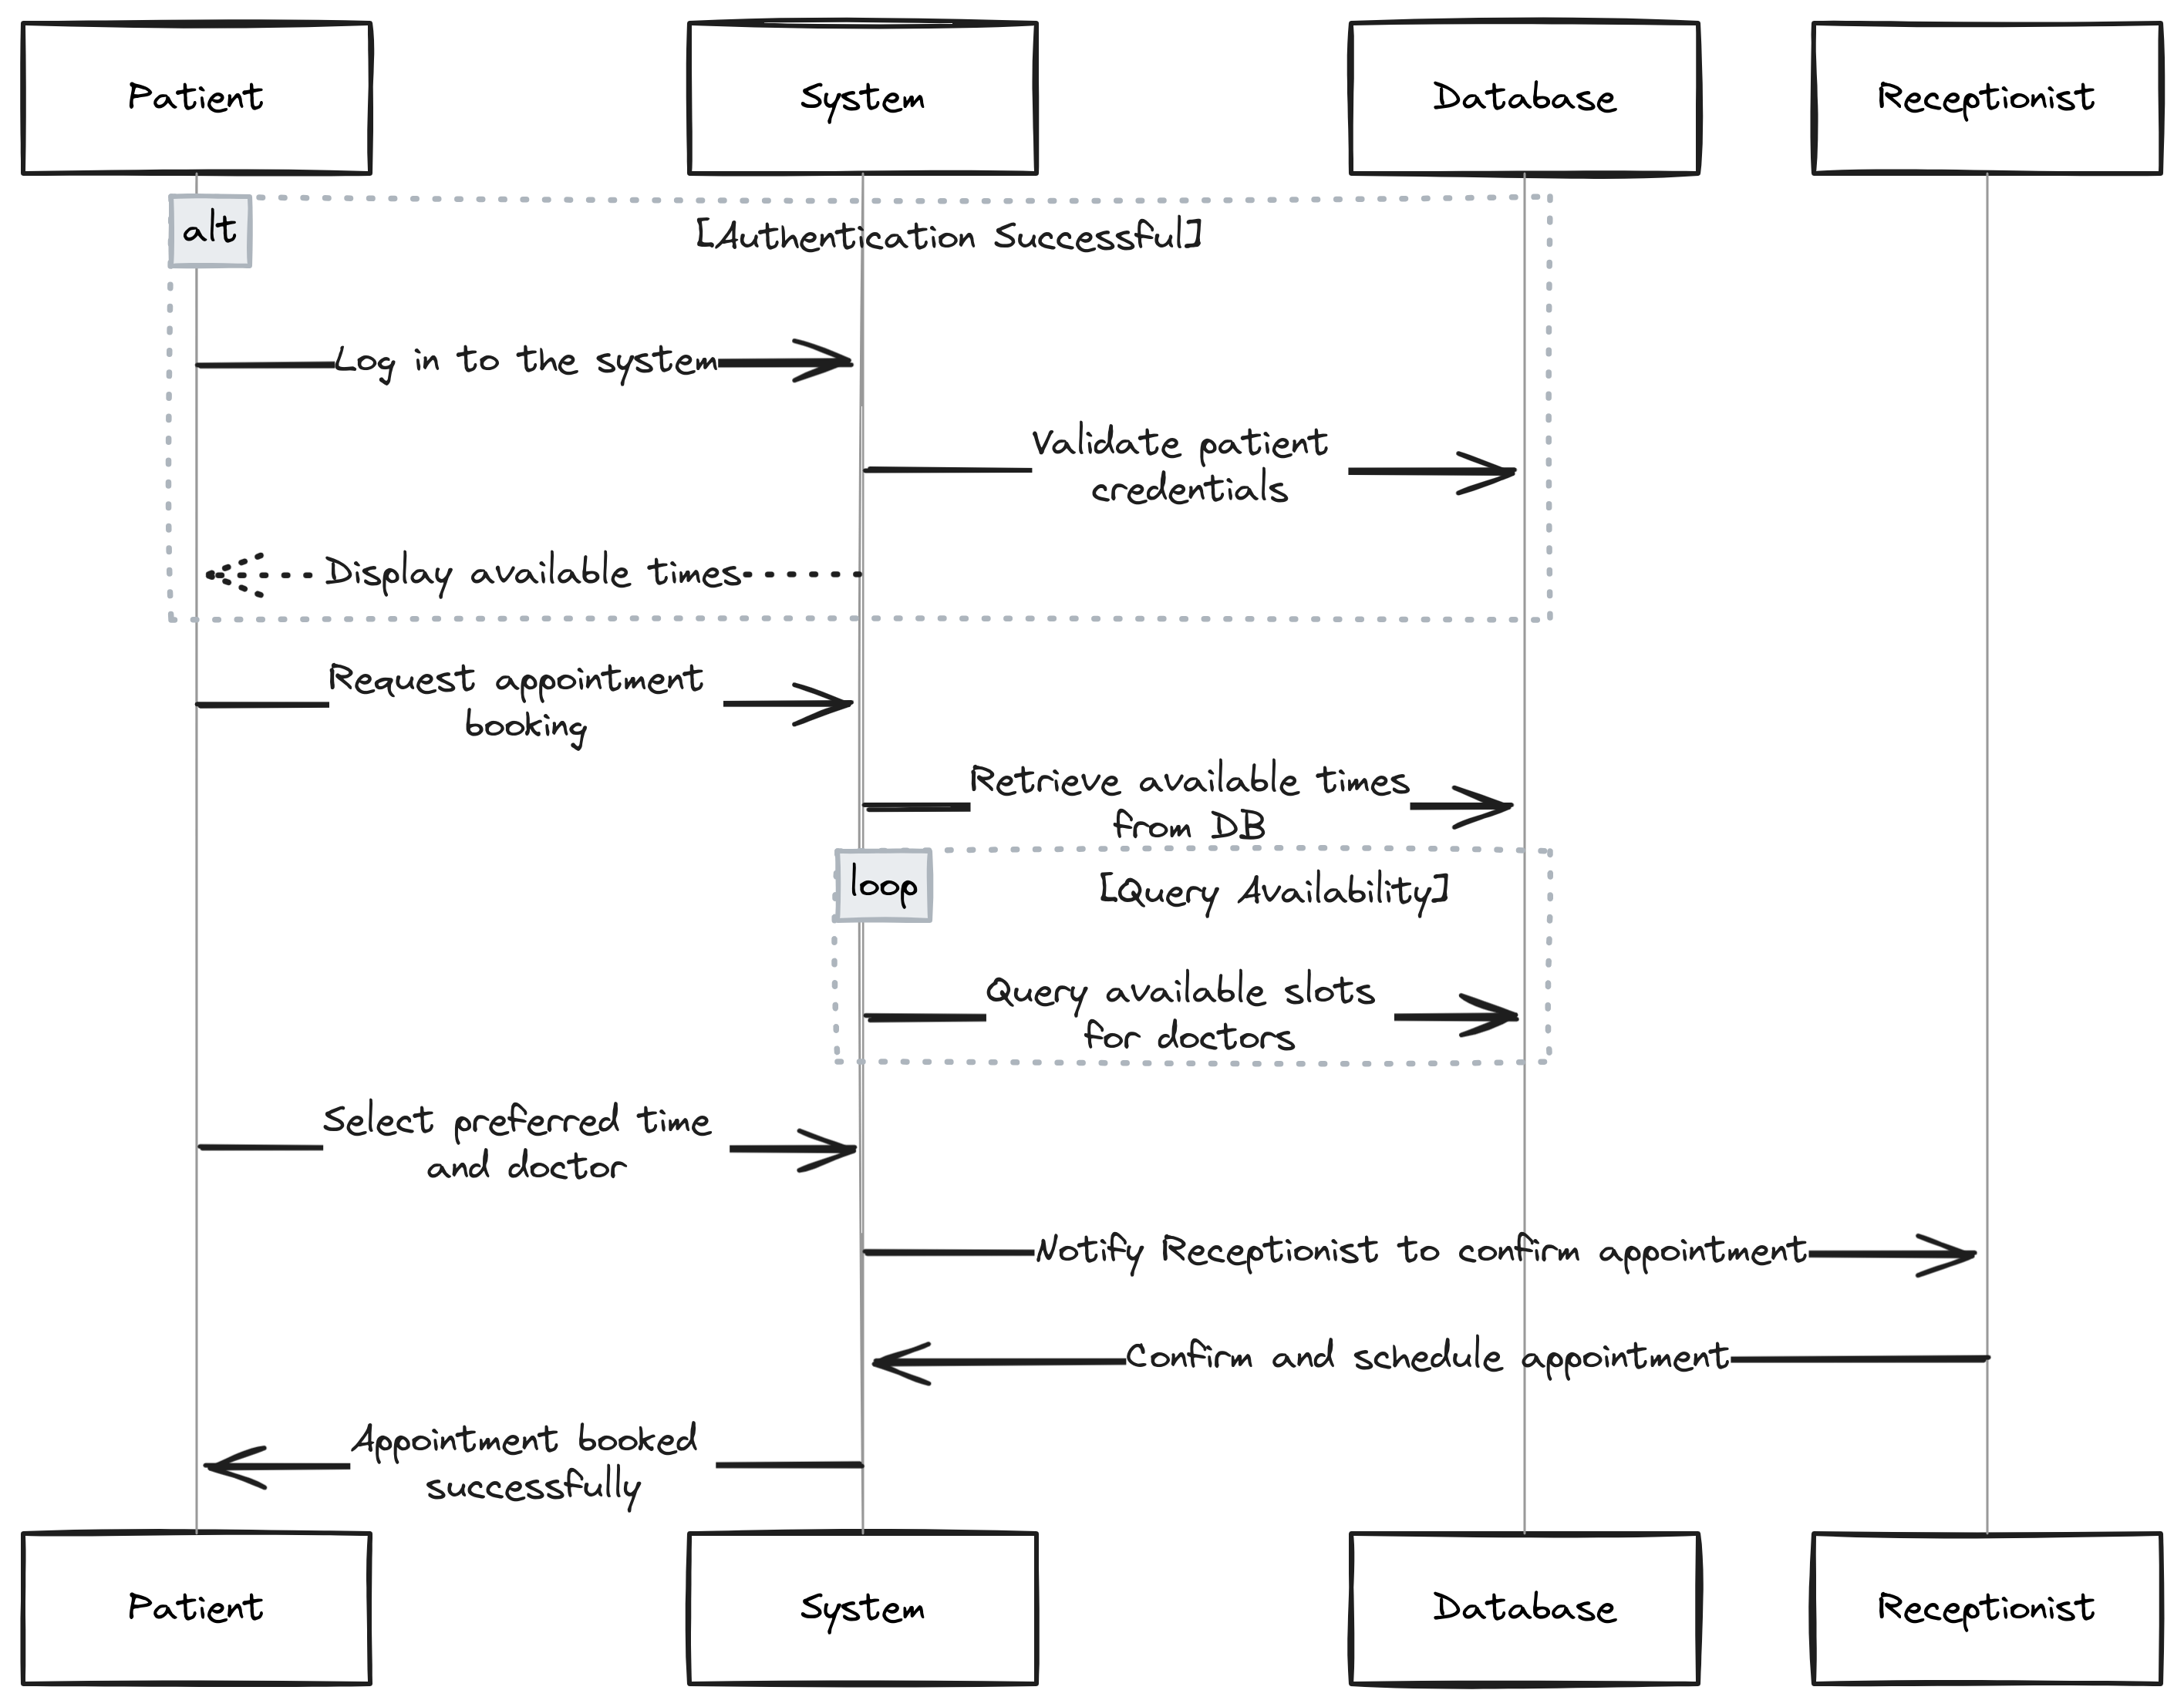
\includegraphics[width=0.8\textwidth]{1.png}
\caption{Revised sequence diagram for Booking an Appointment incorporating SOLID principles}
\end{figure}

\newpage

\subsection*{Medical Consultation}
\begin{figure}[h!]
\centering
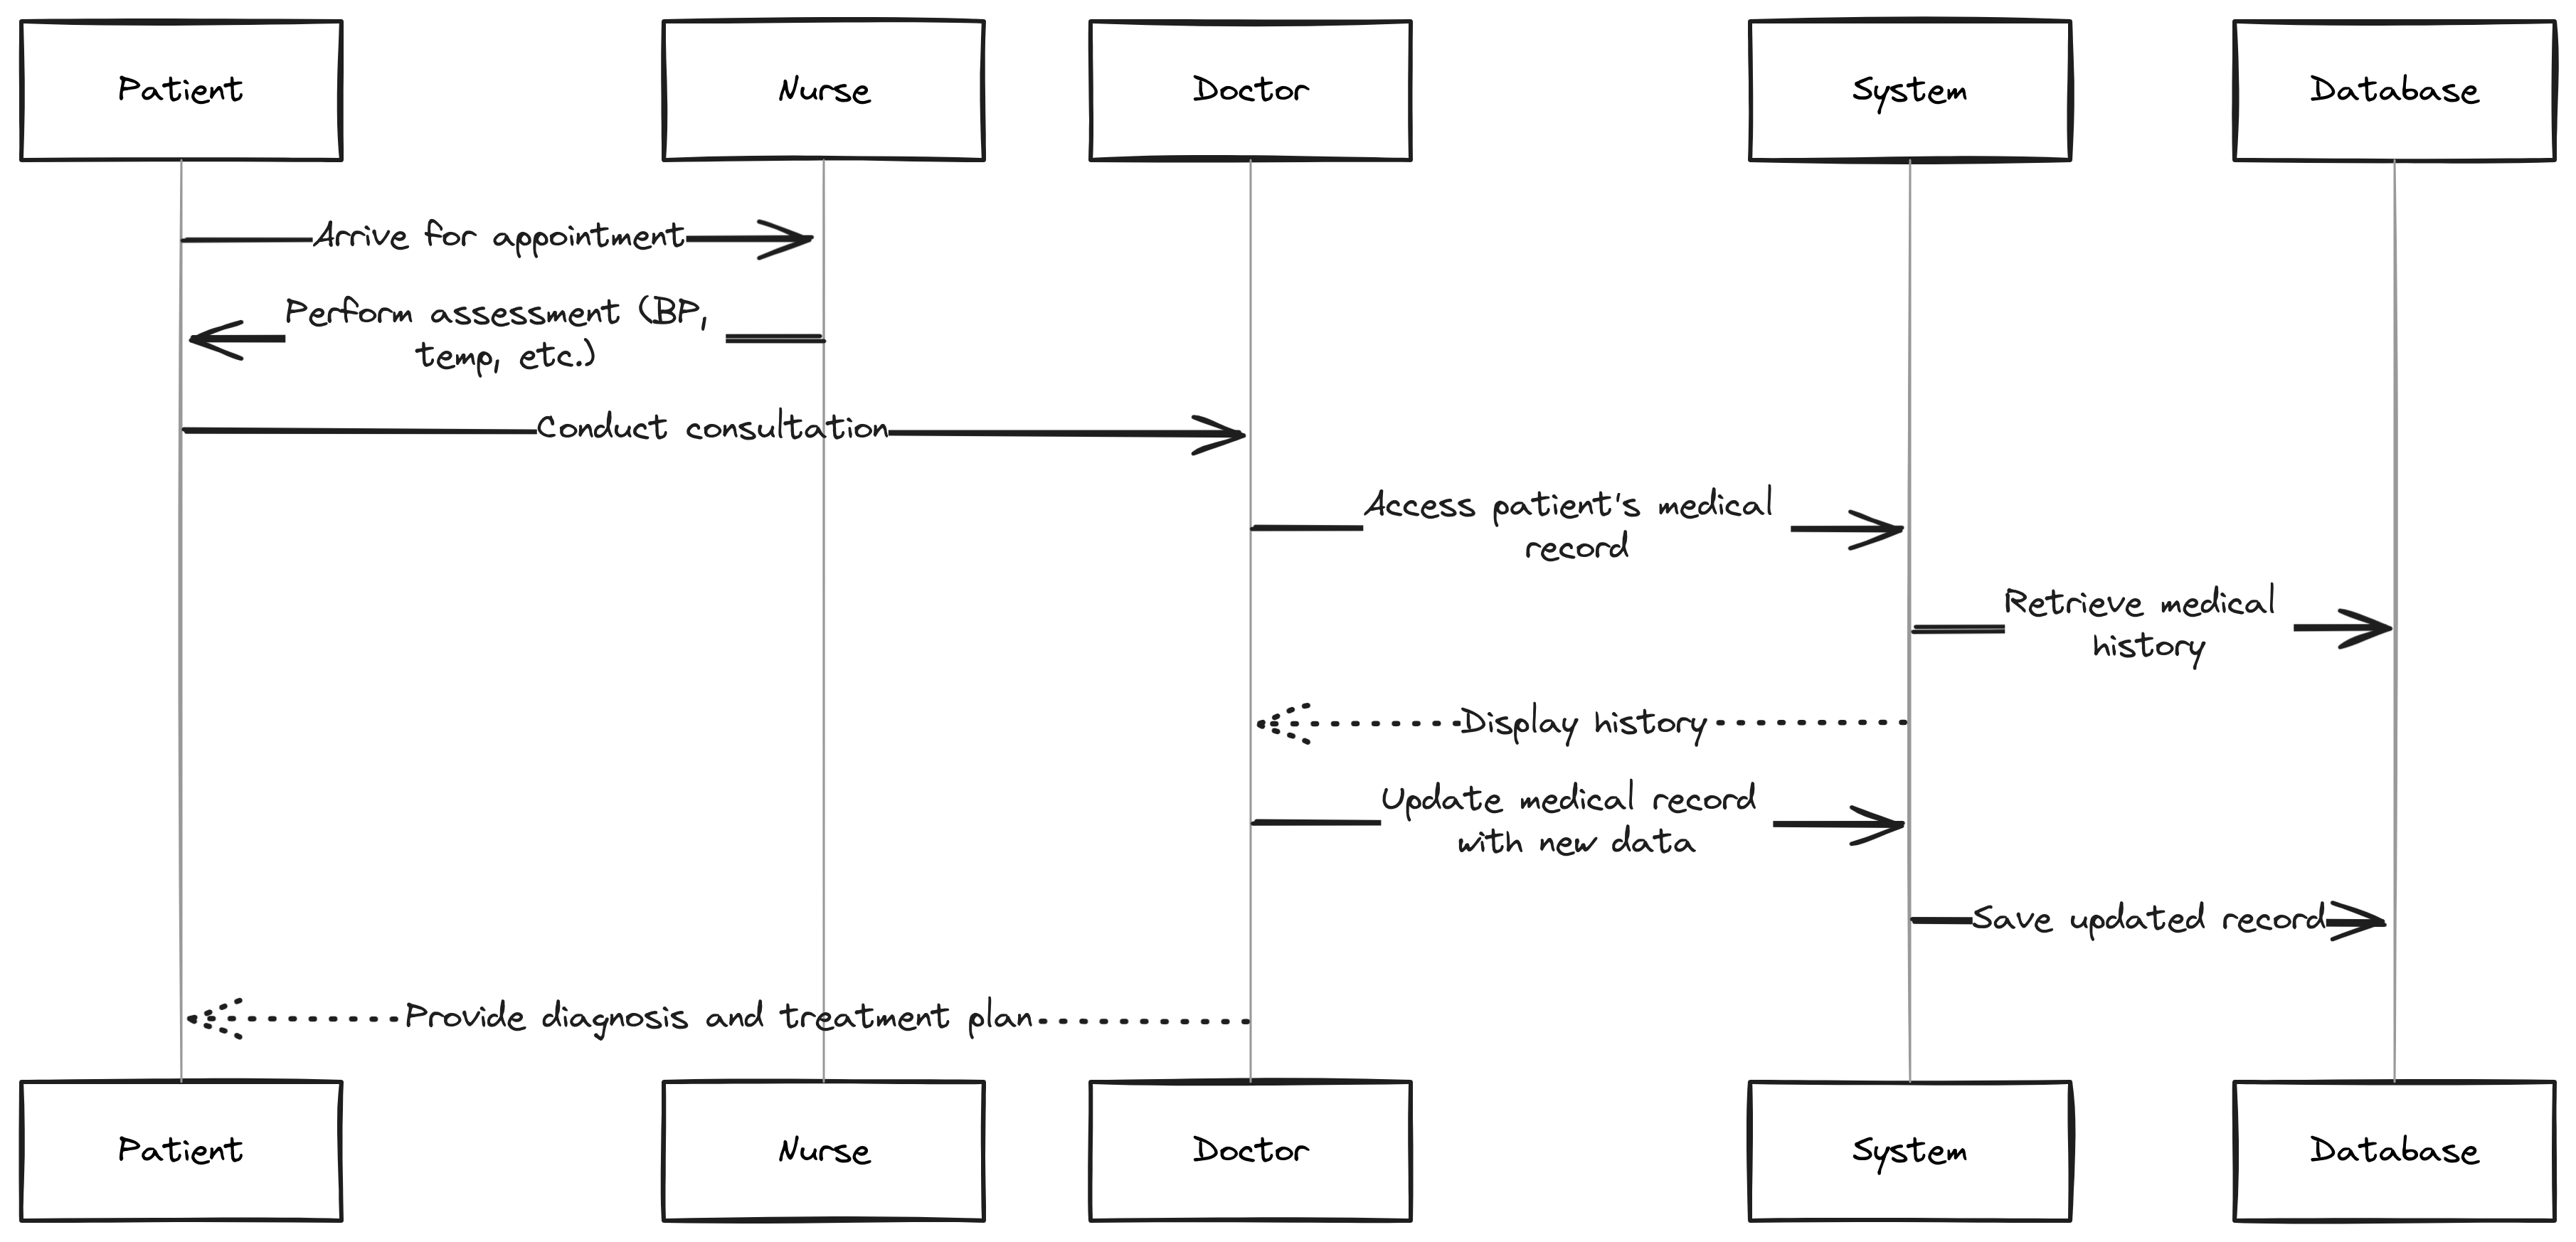
\includegraphics[width=0.8\textwidth]{2.png} % Corrected path if necessary
\caption{Revised sequence diagram for Medical Consultation incorporating SOLID principles}
\end{figure}

\newpage

\subsection*{Patient Registration}
\begin{figure}[h!]
\centering
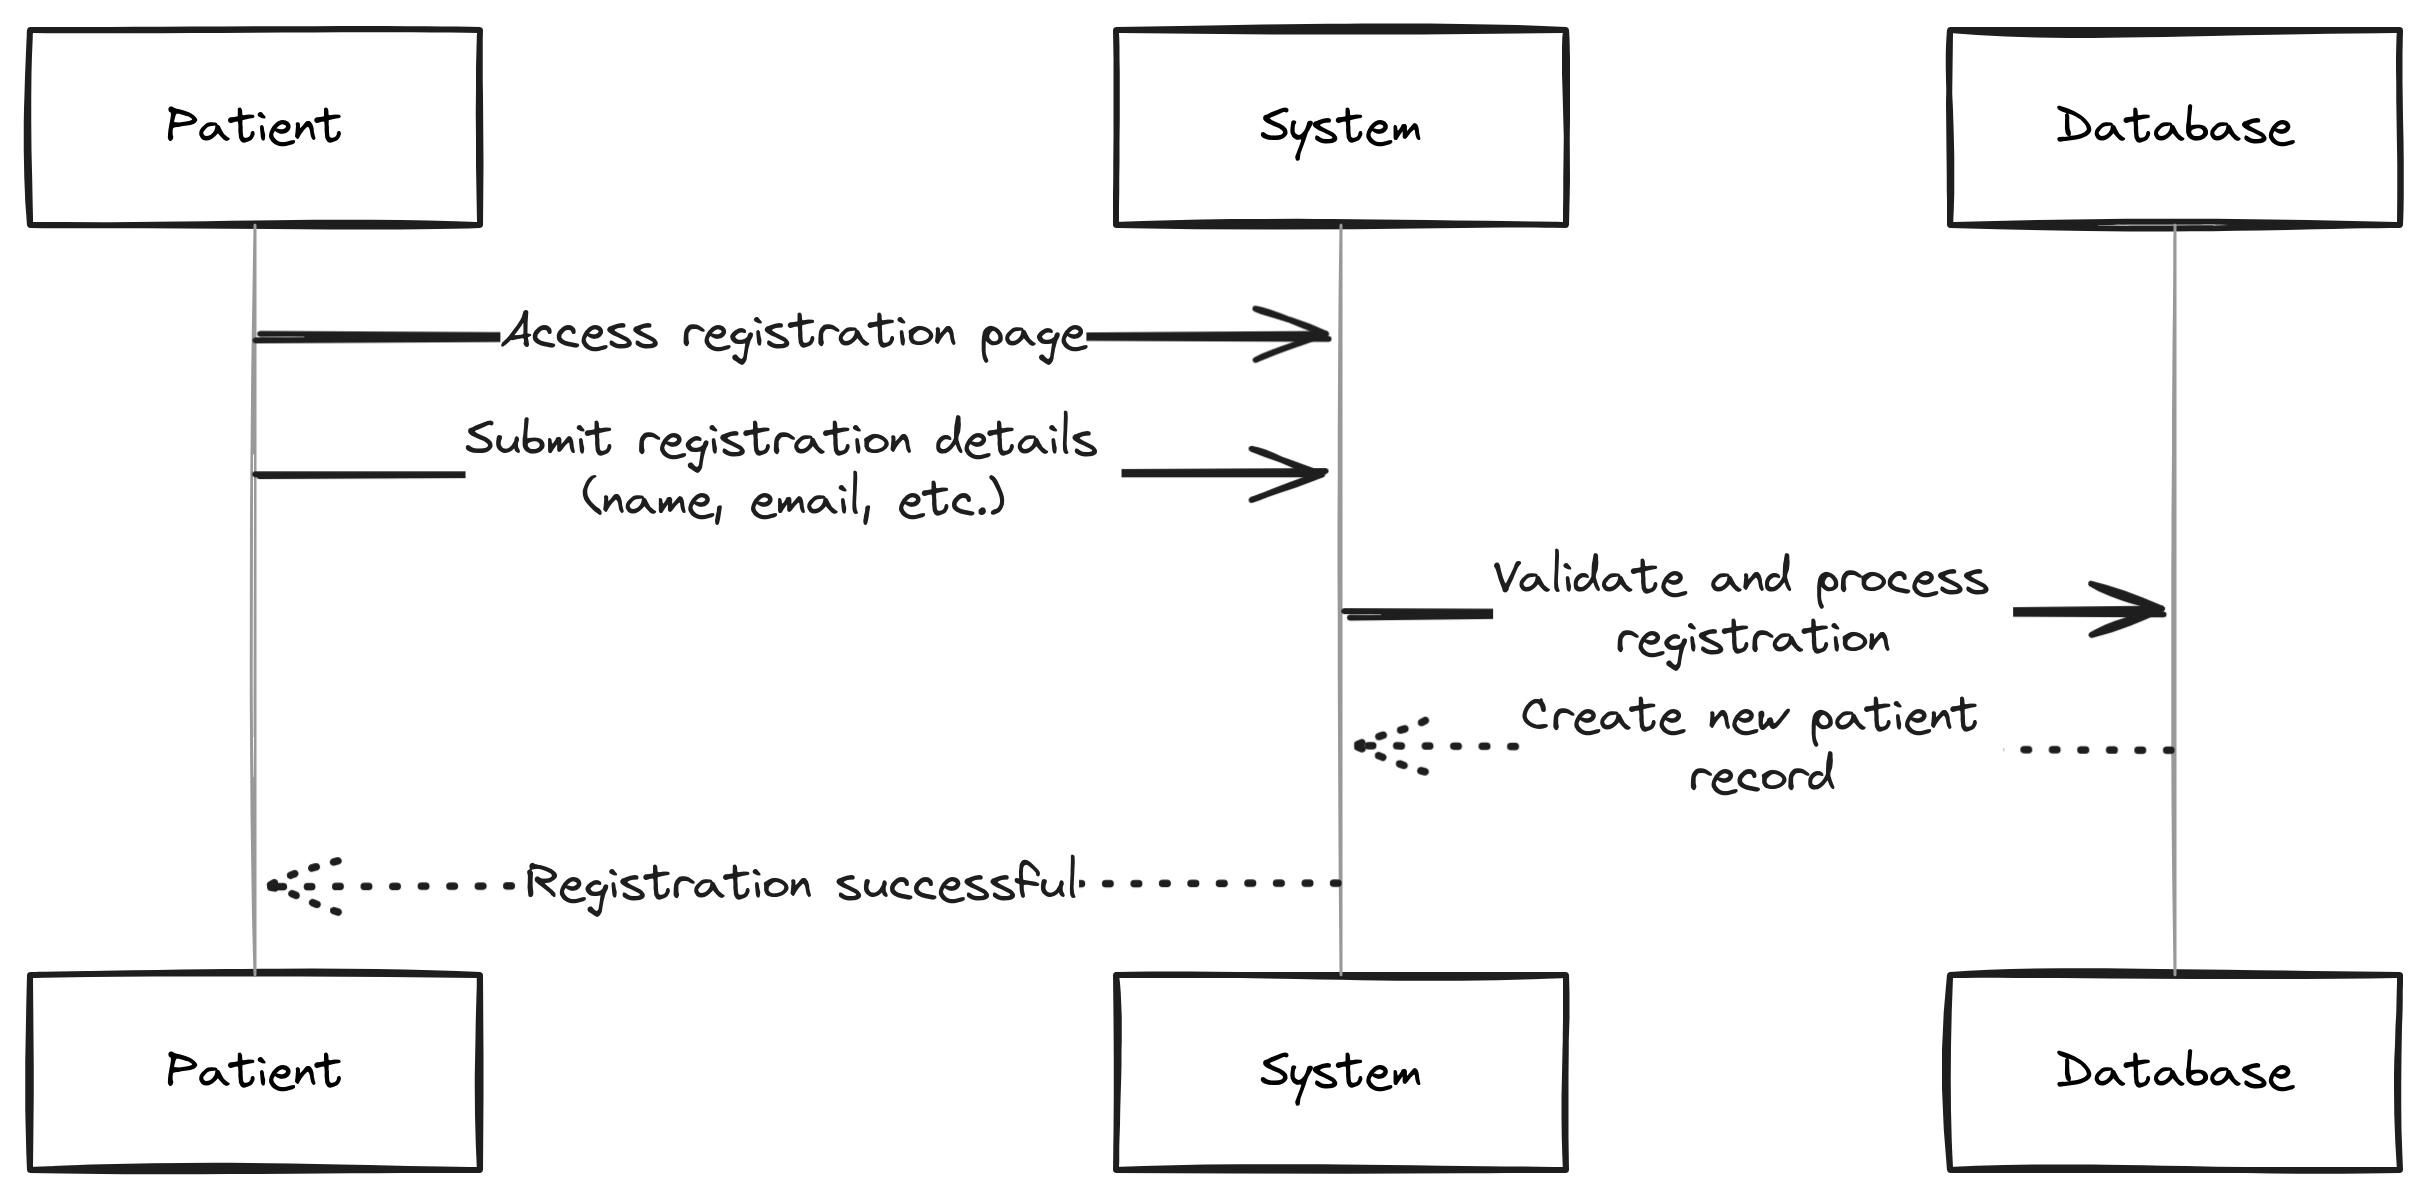
\includegraphics[width=0.8\textwidth]{3.png}
\caption{Revised sequence diagram for Patient Registration incorporating SOLID principles}
\end{figure}

\newpage

\subsection*{Prescription and Pharmacy Interaction}
\begin{figure}[h!]
\centering
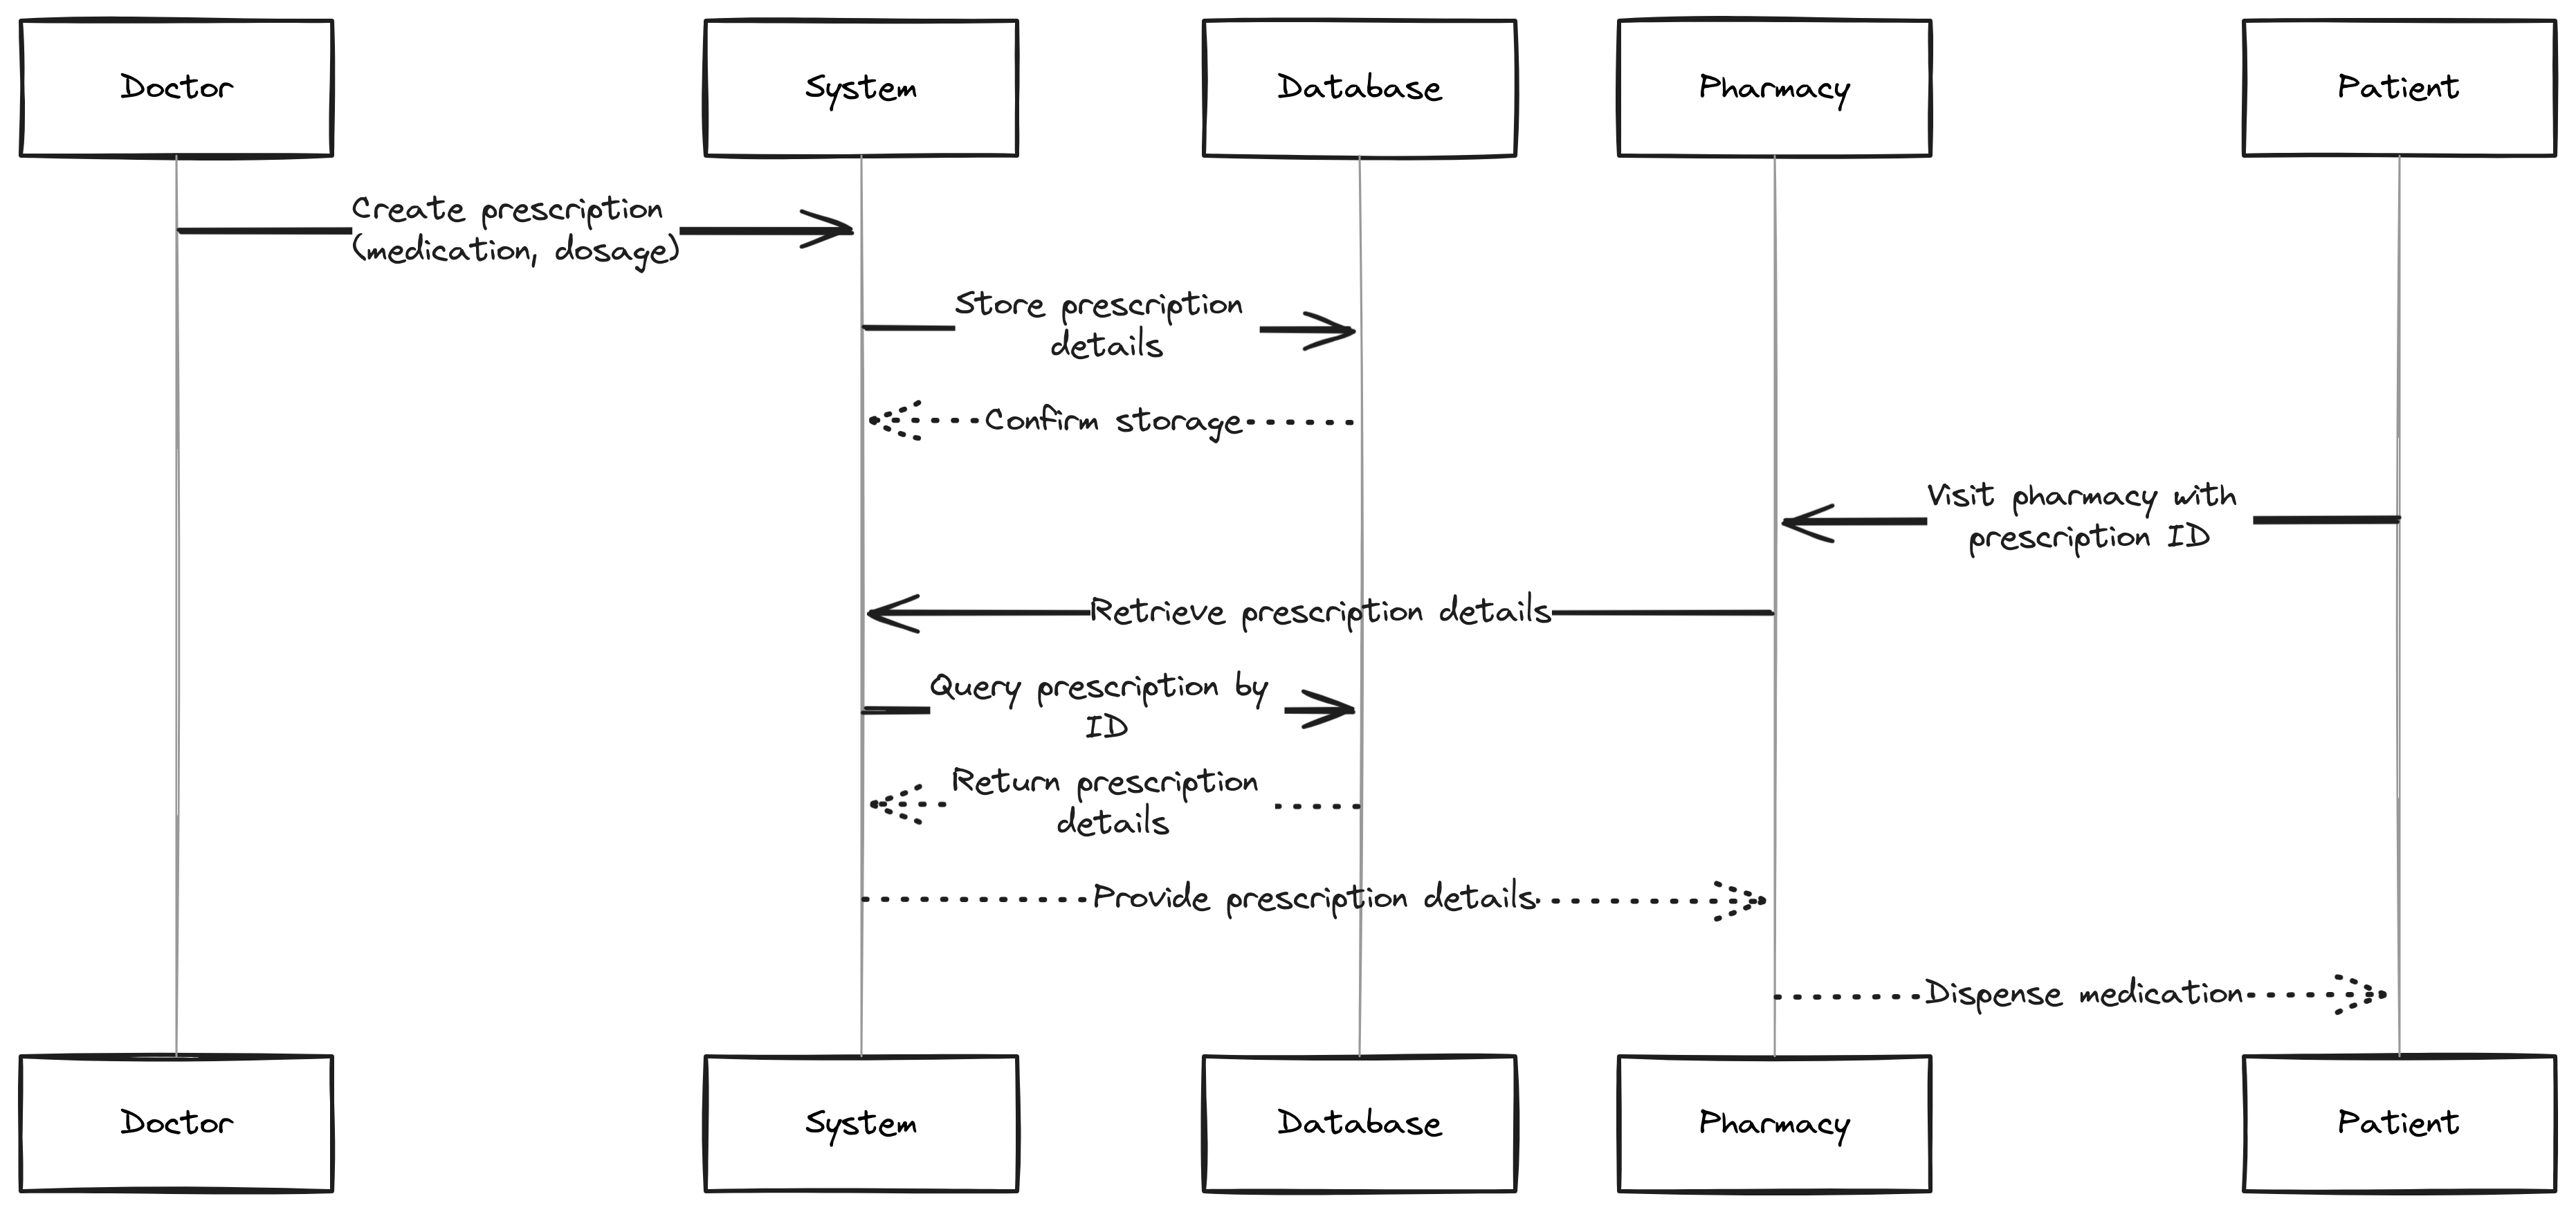
\includegraphics[width=0.8\textwidth]{4.png}
\caption{Revised sequence diagram for Prescription and Pharmacy Interaction incorporating SOLID principles}
\end{figure}


\begin{quote}
    \textbf{\textit{The application of SOLID design principles in the redesign of HMS has significantly improved its architecture. These enhancements not only increase the system's modularity and flexibility but also facilitate future expansions and maintenance efforts.}}
    \end{quote}
    
\end{document}

